\documentclass[11pt,a4paper]{article}

% ===================== PAQUETES =====================
\usepackage[utf8]{inputenc}
\usepackage[T1]{fontenc}
\usepackage[provide=*]{babel}
\babelprovide[main,import]{spanish}
\usepackage{geometry}
\geometry{margin=2.5cm}
\usepackage{graphicx}
\usepackage{listings}
\usepackage{xcolor}
\usepackage{hyperref}
\usepackage{enumitem}
\usepackage{caption}
\usepackage{parskip}
\usepackage{placeins}

\hypersetup{
    colorlinks=true,
    linkcolor=blue,
    urlcolor=blue,
    citecolor=blue
}

% ===================== ESTILO DE CÓDIGO =====================
\definecolor{codebg}{RGB}{245,245,245}
\definecolor{codegray}{RGB}{110,110,110}
\definecolor{codekw}{RGB}{0,0,180}

\lstdefinestyle{codeStyle}{
    backgroundcolor=\color{codebg},
    basicstyle=\ttfamily\small,
    breaklines=true,
    breakatwhitespace=false,
    frame=single,
    numbers=left,
    numberstyle=\tiny\color{codegray},
    keywordstyle=\color{codekw}\bfseries,
    commentstyle=\color{codegray}\itshape,
    tabsize=2,
    showstringspaces=false,
    columns=fullflexible
}
\lstset{style=codeStyle}

% ===================== DATOS DEL DOCUMENTO =====================
\title{\textbf{Práctica Banco-Austro: Implementación de una Base de Datos Distribuida}}
\author{}
\date{}

\begin{document}

\begin{titlepage}
    \centering
    \vspace*{2cm}

    {\Large \textbf{Facultad de Ciencias de la Computación}\par}
    \vspace{0.5cm}
    {\large Materia: Aplicaciones Distribuidas\par}

    \vspace{3cm}

    {\huge \textbf{Práctica: Implementación de una Base de Datos Distribuida para el Banco del Austro}\par}

    \vspace{3cm}

    {\Large \textbf{Estudiante:} Isaias Abraham Urbina Romero\par}

    \vfill

    {\large 14 de julio de 2026\par}

\end{titlepage}

% ===================== INTRODUCCIÓN =====================
\section*{Introducción}

Las bases de datos distribuidas permiten almacenar información en diferentes servidores físicos o lógicos, ofreciendo mayor disponibilidad, escalabilidad y tolerancia a fallos. En este tipo de arquitectura, los datos se encuentran fragmentados o replicados entre varios nodos, mientras que el usuario interactúa con el sistema como si se tratara de una única base de datos.

En la presente práctica se desarrolló una aplicación distribuida para el Banco del Austro utilizando Spring Boot, PostgreSQL y Docker. Se implementaron dos nodos de base de datos correspondientes a las oficinas de Cuenca y Quito, cada uno con su propia información de clientes, cuentas y transacciones. La aplicación determina automáticamente a qué base de datos conectarse mediante el prefijo del número de cuenta, permitiendo realizar consultas de manera transparente para el usuario.

% ===================== OBJETIVOS =====================
\FloatBarrier
\section{Objetivos}

\subsection*{Objetivo general}

Desarrollar una aplicación distribuida utilizando Spring Boot y PostgreSQL que permita consultar información bancaria almacenada en dos nodos independientes, aplicando técnicas de fragmentación horizontal y enrutamiento de consultas.

\subsection*{Objetivos específicos}

\begin{itemize}[leftmargin=*]
    \item Configurar dos bases de datos PostgreSQL mediante contenedores Docker.
    \item Implementar múltiples conexiones (DataSource) dentro de Spring Boot.
    \item Enrutar automáticamente las consultas hacia el nodo correspondiente según el prefijo del número de cuenta.
    \item Realizar consultas distribuidas que permitan obtener información desde ambos nodos.
    \item Verificar el funcionamiento de la aplicación mediante pruebas de los servicios REST.
\end{itemize}

% ===================== DESARROLLO =====================
\FloatBarrier
\section{Desarrollo}

\FloatBarrier
\subsection{Creación del proyecto}

Para el desarrollo de la aplicación se creó un proyecto utilizando Spring Boot, administrado mediante Maven. La estructura del proyecto se organizó siguiendo la arquitectura propuesta por Spring, separando la configuración, la lógica del negocio y los controladores REST en paquetes independientes.

La aplicación fue desarrollada en Java y utiliza el framework Spring Boot para facilitar la creación de servicios web y la administración de múltiples conexiones hacia diferentes bases de datos PostgreSQL.

\begin{figure}[h!]
    \centering
    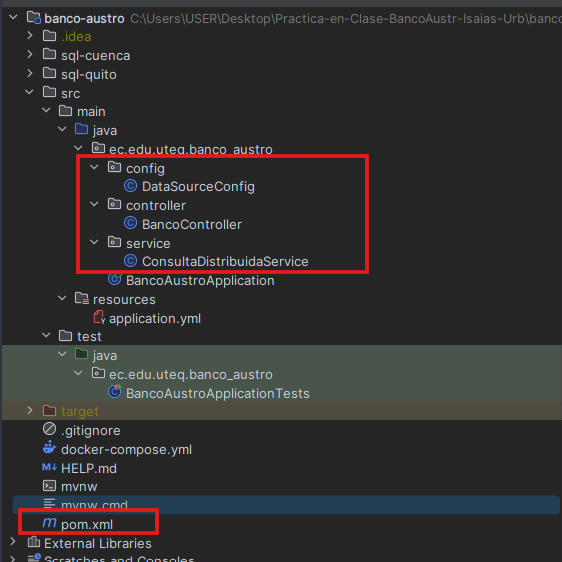
\includegraphics[width=0.55\textwidth]{images/image1.png}
    \caption{Estructura del Proyecto}
\end{figure}

\FloatBarrier
\subsection{Configuración de los nodos PostgreSQL mediante Docker}

Con el propósito de simular una base de datos distribuida, se implementaron dos nodos PostgreSQL utilizando contenedores Docker. Cada nodo representa una oficina diferente del Banco del Austro:

\begin{itemize}[leftmargin=*]
    \item Nodo Cuenca, encargado de almacenar la información correspondiente a las cuentas cuyo prefijo es 22.
    \item Nodo Quito, encargado de almacenar la información correspondiente a las cuentas cuyo prefijo es 17.
\end{itemize}

Cada contenedor posee una base de datos independiente con sus propias tablas y registros iniciales. La creación automática de las estructuras y los datos se realizó mediante scripts SQL ejecutados durante el inicio de cada contenedor.

La configuración de ambos servicios se definió en el archivo \texttt{docker-compose.yml}, donde se especificaron las imágenes utilizadas, credenciales de acceso, puertos, volúmenes persistentes y las carpetas que contienen los scripts de inicialización (a continuación el código del \texttt{docker-compose.yml}):

\begin{lstlisting}[caption={docker-compose.yml}]
services:

  db-cuenca:
    image: postgres:16-alpine
    container_name: banco-cuenca
    environment:
      POSTGRES_DB: banco_cuenca
      POSTGRES_USER: banco
      POSTGRES_PASSWORD: banco123
    ports:
      - "5442:5432"
    volumes:
      - vol-cuenca:/var/lib/postgresql/data
      - ./sql-cuenca:/docker-entrypoint-initdb.d
    networks:
      - bda-net

  db-quito:
    image: postgres:16-alpine
    container_name: banco-quito
    environment:
      POSTGRES_DB: banco_quito
      POSTGRES_USER: banco
      POSTGRES_PASSWORD: banco123
    ports:
      - "5433:5432"
    volumes:
      - vol-quito:/var/lib/postgresql/data
      - ./sql-quito:/docker-entrypoint-initdb.d
    networks:
      - bda-net

networks:
  bda-net:
    driver: bridge

volumes:
  vol-cuenca:
  vol-quito:
\end{lstlisting}

Una vez configurados los contenedores, se inició el entorno utilizando Docker Compose. Al ejecutar el comando correspondiente se verificó que ambos nodos se encontraban activos y escuchando en diferentes puertos:

\begin{itemize}[leftmargin=*]
    \item Cuenca: puerto 5442 (ajustado para evitar conflicto con otra instalación de PostgreSQL).
    \item Quito: puerto 5433.
\end{itemize}

Esto permitió que la aplicación pudiera conectarse de forma independiente a cada base de datos.

\begin{figure}[h!]
    \centering
    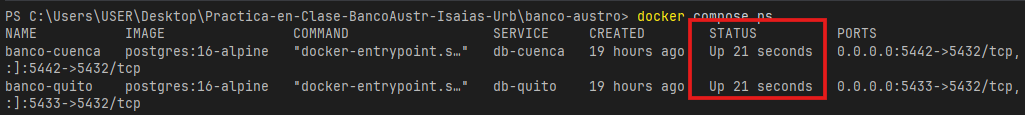
\includegraphics[width=0.85\textwidth]{images/image2.png}
    \caption{Resultado de \texttt{docker compose ps}}
\end{figure}

\FloatBarrier
\subsection{Creación de las bases de datos}

Cada nodo contiene tres tablas principales:

\begin{itemize}[leftmargin=*]
    \item \textbf{clientes}, donde se almacena la información personal de cada cliente.
    \item \textbf{cuentas}, que registra el número de cuenta, el saldo disponible y la oficina a la que pertenece.
    \item \textbf{transacciones}, utilizada para almacenar el historial de movimientos realizados.
\end{itemize}

La estructura de las tablas es similar en ambos nodos; sin embargo, cada base de datos almacena únicamente la información correspondiente a su oficina. De esta manera se implementa una fragmentación horizontal por ubicación geográfica, donde cada servidor administra únicamente una parte de la información total del sistema.

\begin{lstlisting}[language=SQL, caption={01\_schema.sql -- Cuenca}]
CREATE TABLE IF NOT EXISTS clientes (
  id BIGSERIAL PRIMARY KEY,
  cedula VARCHAR(10) UNIQUE NOT NULL,
  nombre VARCHAR(120) NOT NULL,
  ciudad VARCHAR(60) NOT NULL,
  creado_en TIMESTAMP NOT NULL DEFAULT NOW()
);

CREATE TABLE IF NOT EXISTS cuentas (
  id BIGSERIAL PRIMARY KEY,
  numero VARCHAR(20) UNIQUE NOT NULL,
  cliente_id BIGINT NOT NULL REFERENCES clientes(id),
  saldo NUMERIC(15,2) NOT NULL DEFAULT 0.00
    CHECK (saldo >= 0),
  oficina VARCHAR(20) NOT NULL CHECK (oficina = 'CUENCA'),
  abierta_en TIMESTAMP NOT NULL DEFAULT NOW()
);

CREATE TABLE IF NOT EXISTS transacciones (
  id BIGSERIAL PRIMARY KEY,
  cuenta_orig VARCHAR(20) NOT NULL,
  cuenta_dest VARCHAR(20) NOT NULL,
  monto NUMERIC(15,2) NOT NULL CHECK (monto > 0),
  fecha TIMESTAMP NOT NULL DEFAULT NOW(),
  estado VARCHAR(20) NOT NULL DEFAULT 'COMPLETADA',
  oficina VARCHAR(20) NOT NULL CHECK (oficina = 'CUENCA')
);

CREATE INDEX idx_cuentas_cliente ON cuentas(cliente_id);
CREATE INDEX idx_transacciones_orig ON transacciones(cuenta_orig);
CREATE INDEX idx_transacciones_fecha ON transacciones(fecha);
\end{lstlisting}

\begin{lstlisting}[language=SQL, caption={02\_datos.sql -- Cuenca}]
INSERT INTO clientes (cedula, nombre, ciudad) VALUES
('0101234567', 'Mario Vintimilla', 'Cuenca'),
('0107654321', 'Sofia Vasquez', 'Cuenca'),
('0103456789', 'Andres Cordero', 'Cuenca');

INSERT INTO cuentas (numero, cliente_id, saldo, oficina) VALUES
('2201000001', 1, 15000.00, 'CUENCA'),
('2201000002', 2, 4200.50, 'CUENCA'),
('2201000003', 3, 850.75, 'CUENCA');

INSERT INTO transacciones (cuenta_orig, cuenta_dest, monto, oficina) VALUES
('2201000001', '2201000002', 500.00, 'CUENCA'),
('2201000002', '2201000003', 120.25, 'CUENCA');
\end{lstlisting}

\FloatBarrier
\subsection{Configuración de Spring Boot}

\subsubsection*{Configuración del archivo application.yml}

Para permitir la conexión con las dos bases de datos distribuidas, se configuró el archivo \texttt{application.yml}. En este archivo se definieron dos orígenes de datos (DataSource): uno para la oficina de Cuenca y otro para la oficina de Quito.

Cada conexión contiene la dirección de la base de datos, el usuario, la contraseña y el controlador JDBC de PostgreSQL. Debido a un conflicto con una instalación local de PostgreSQL, el nodo de Cuenca fue configurado para utilizar el puerto 5442, mientras que el nodo de Quito utiliza el puerto 5433.

Esta configuración permite que la aplicación pueda establecer conexiones independientes hacia cada nodo según sea necesario.

\begin{figure}[h!]
    \centering
    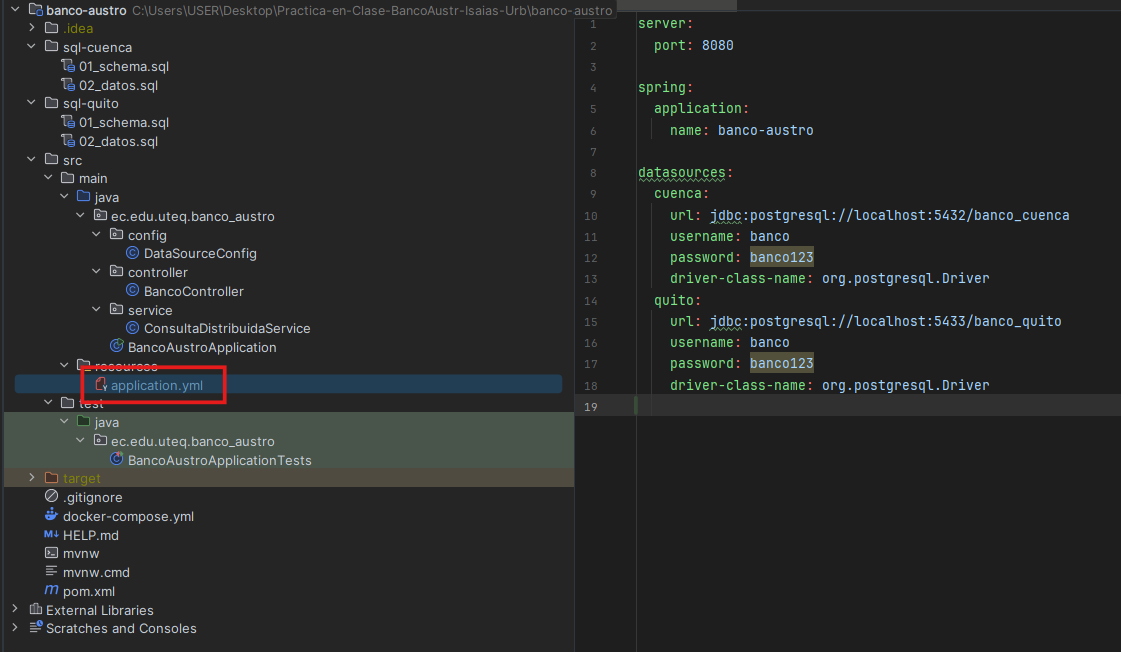
\includegraphics[width=0.75\textwidth]{images/image3.png}
    \caption{Captura del archivo application.yml}
\end{figure}

\FloatBarrier
\subsection{Configuración de los DataSource}

Una vez definidas las conexiones en el archivo de configuración, se implementó la clase \texttt{DataSourceConfig}, encargada de crear los dos objetos DataSource que utilizará la aplicación.

Cada objeto representa una conexión independiente hacia una base de datos diferente y posteriormente es utilizado por el servicio para ejecutar las consultas correspondientes. Esta separación facilita la administración de múltiples bases de datos dentro de una misma aplicación Spring Boot.

Durante el inicio de la aplicación se imprimen en la consola las direcciones de conexión de ambos nodos, permitiendo verificar que la configuración fue cargada correctamente.

\begin{lstlisting}[language=Java, caption={DataSourceConfig.java}]
package ec.edu.uteq.banco_austro.config;

import javax.sql.DataSource;
import org.springframework.beans.factory.annotation.Value;
import org.springframework.boot.jdbc.DataSourceBuilder;
import org.springframework.context.annotation.Bean;
import org.springframework.context.annotation.Configuration;

@Configuration
public class DataSourceConfig {

    @Value("${datasources.cuenca.url}")
    private String cuencaUrl;

    @Value("${datasources.cuenca.username}")
    private String cuencaUser;

    @Value("${datasources.cuenca.password}")
    private String cuencaPass;

    @Value("${datasources.quito.url}")
    private String quitoUrl;

    @Value("${datasources.quito.username}")
    private String quitoUser;

    @Value("${datasources.quito.password}")
    private String quitoPass;

    @Bean(name = "dsCuenca")
    public DataSource dsCuenca() {

        System.out.println("===== CONFIGURACION CUENCA =====");
        System.out.println("URL : " + cuencaUrl);
        System.out.println("USER : " + cuencaUser);
        System.out.println("PASS : " + cuencaPass);

        return DataSourceBuilder.create()
                .url(cuencaUrl)
                .username(cuencaUser)
                .password(cuencaPass)
                .driverClassName("org.postgresql.Driver")
                .build();
    }

    @Bean(name = "dsQuito")
    public DataSource dsQuito() {

        System.out.println("===== CONFIGURACION QUITO =====");
        System.out.println("URL : " + quitoUrl);
        System.out.println("USER : " + quitoUser);
        System.out.println("PASS : " + quitoPass);

        return DataSourceBuilder.create()
                .url(quitoUrl)
                .username(quitoUser)
                .password(quitoPass)
                .driverClassName("org.postgresql.Driver")
                .build();
    }
}
\end{lstlisting}

\FloatBarrier
\subsection{Implementación del servicio distribuido}

La lógica principal del sistema fue implementada en la clase \texttt{ConsultaDistribuidaService}, responsable de determinar automáticamente a qué base de datos debe dirigirse cada consulta.

Para ello, la aplicación analiza los dos primeros dígitos del número de cuenta ingresado por el usuario.

\begin{itemize}[leftmargin=*]
    \item Si el número comienza con 22, la consulta es enviada al nodo correspondiente a Cuenca.
    \item Si el número comienza con 17, la consulta es enviada al nodo correspondiente a Quito.
\end{itemize}

Este mecanismo de enrutamiento permite que el usuario no necesite conocer la ubicación física de la información, ya que la aplicación selecciona automáticamente la base de datos adecuada.

Además del enrutamiento por prefijo, el servicio implementa una consulta que obtiene la lista completa de clientes combinando la información almacenada en ambos nodos. Para ello, primero consulta la base de datos de Cuenca y posteriormente la de Quito, uniendo los resultados en una sola colección que es enviada al cliente.

Esta estrategia demuestra el funcionamiento de una consulta distribuida, donde la información se obtiene desde diferentes servidores y se presenta de forma unificada.

\begin{lstlisting}[language=Java, caption={ConsultaDistribuidaService.java}]
package ec.edu.uteq.banco_austro.service;

import java.util.ArrayList;
import java.util.List;
import java.util.Map;
import javax.sql.DataSource;
import org.springframework.beans.factory.annotation.Qualifier;
import org.springframework.jdbc.core.JdbcTemplate;
import org.springframework.stereotype.Service;

@Service
public class ConsultaDistribuidaService {

    private final JdbcTemplate jdbcCuenca;
    private final JdbcTemplate jdbcQuito;

    public ConsultaDistribuidaService(
            @Qualifier("dsCuenca") DataSource dsCuenca,
            @Qualifier("dsQuito") DataSource dsQuito) {
        this.jdbcCuenca = new JdbcTemplate(dsCuenca);
        this.jdbcQuito = new JdbcTemplate(dsQuito);
    }

    public Map<String, Object> consultarSaldo(String numero) {
        JdbcTemplate destino = enrutar(numero);
        String sql = "SELECT numero, saldo, oficina "
                + "FROM cuentas WHERE numero = ?";
        List<Map<String, Object>> filas =
                destino.queryForList(sql, numero);
        if (filas.isEmpty()) {
            return Map.of(
                    "error", "Cuenta no encontrada",
                    "numero", numero);
        }
        return filas.get(0);
    }

    public List<Map<String, Object>> listarTodosLosClientes() {
        String sql = "SELECT cedula, nombre, ciudad FROM clientes";
        List<Map<String, Object>> union = new ArrayList<>();
        union.addAll(jdbcCuenca.queryForList(sql));
        union.addAll(jdbcQuito.queryForList(sql));
        return union;
    }

    private JdbcTemplate enrutar(String numero) {
        if (numero == null || numero.length() < 2) {
            throw new IllegalArgumentException(
                    "Numero de cuenta invalido: " + numero);
        }
        String prefijo = numero.substring(0, 2);
        return switch (prefijo) {
            case "22" -> jdbcCuenca;
            case "17" -> jdbcQuito;
            default -> throw new IllegalArgumentException(
                    "Prefijo de oficina no reconocido: " + prefijo);
        };
    }
}
\end{lstlisting}

\FloatBarrier
\subsection{Implementación del controlador REST}

Para exponer la funcionalidad de la aplicación se implementó la clase \texttt{BancoController}, la cual define los servicios REST disponibles para los usuarios.

Se desarrollaron dos endpoints principales:

\begin{itemize}[leftmargin=*]
    \item \textbf{Consultar saldo}, que recibe el número de cuenta y devuelve la información correspondiente al nodo donde se encuentra almacenada.
    \item \textbf{Listar clientes}, que obtiene los registros existentes en ambas bases de datos y los presenta como una única respuesta.
\end{itemize}

El controlador recibe las solicitudes HTTP, delega el procesamiento al servicio distribuido y devuelve la información en formato JSON.

\begin{lstlisting}[language=Java, caption={BancoController.java}]
package ec.edu.uteq.banco_austro.controller;

import java.util.List;
import java.util.Map;
import ec.edu.uteq.banco_austro.service.ConsultaDistribuidaService;
import org.springframework.web.bind.annotation.GetMapping;
import org.springframework.web.bind.annotation.PathVariable;
import org.springframework.web.bind.annotation.RequestMapping;
import org.springframework.web.bind.annotation.RestController;

@RestController
@RequestMapping("/api/banco")
public class BancoController {

    private final ConsultaDistribuidaService service;

    public BancoController(ConsultaDistribuidaService service) {
        this.service = service;
    }

    @GetMapping("/saldo/{numero}")
    public Map<String, Object> saldo(@PathVariable String numero) {
        return service.consultarSaldo(numero);
    }

    @GetMapping("/clientes")
    public List<Map<String, Object>> clientes() {
        return service.listarTodosLosClientes();
    }
}
\end{lstlisting}

\FloatBarrier
\subsection{Ejecución de la aplicación}

Una vez configurados los contenedores Docker y desarrollada la aplicación en Spring Boot, se procedió a ejecutar el proyecto desde el entorno de desarrollo IntelliJ IDEA.

Durante el inicio de la aplicación se verificó la correcta carga de los dos orígenes de datos configurados para las oficinas de Cuenca y Quito. Posteriormente, Spring Boot inicializó el servidor web embebido Tomcat en el puerto 8080, permitiendo el acceso a los servicios REST implementados.

Además, se comprobó que ambos grupos de conexiones (HikariPool) lograron establecer comunicación con las bases de datos correspondientes, confirmando que la configuración distribuida funcionó correctamente.

\begin{figure}[h!]
    \centering
    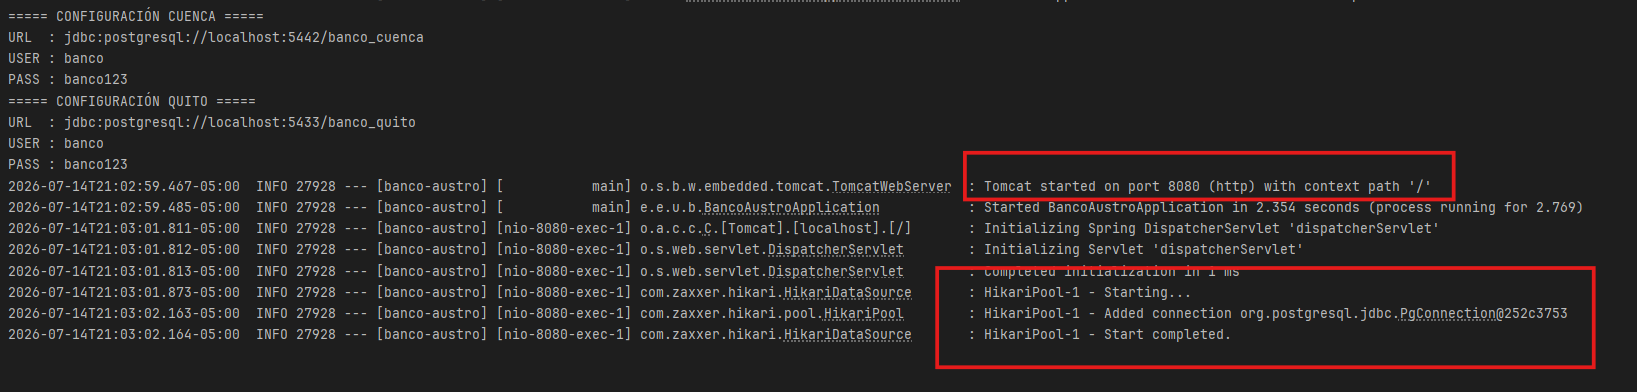
\includegraphics[width=0.85\textwidth]{images/image4.png}
    \caption{Inicio exitoso de la aplicación Banco Austro, mostrando el arranque del servidor Tomcat en el puerto 8080 y la inicialización del pool de conexiones HikariCP hacia la base de datos PostgreSQL.}
\end{figure}

% ===================== PRUEBAS REALIZADAS =====================
\FloatBarrier
\section{Pruebas realizadas}

\FloatBarrier
\subsection{Consulta de una cuenta perteneciente a Cuenca}

Se realizó una consulta utilizando el endpoint encargado de obtener la información de una cuenta bancaria. Se ingresó el número de cuenta 2201000001, cuyo prefijo corresponde a la oficina de Cuenca.

La aplicación identificó automáticamente el prefijo 22 y direccionó la consulta hacia la base de datos del nodo Cuenca. Como resultado, se obtuvo correctamente el número de cuenta, el saldo disponible y la oficina a la que pertenece.

Endpoint utilizado: \texttt{GET /api/banco/saldo/2201000001}

\begin{figure}[h!]
    \centering
    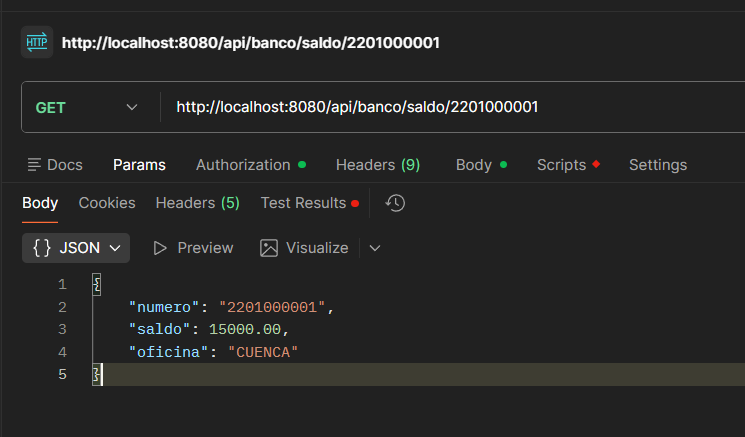
\includegraphics[width=0.7\textwidth]{images/image5.png}
    \caption{Captura de Postman mostrando la respuesta JSON.}
\end{figure}

\FloatBarrier
\subsection{Consulta de una cuenta perteneciente a Quito}

Posteriormente se consultó una cuenta registrada en el nodo Quito mediante el número 1701000001.

En este caso, la aplicación detectó el prefijo 17 y dirigió automáticamente la consulta hacia la segunda base de datos. La información obtenida correspondió correctamente a la cuenta almacenada en dicho nodo.

Endpoint utilizado: \texttt{GET /api/banco/saldo/1701000001}

\begin{figure}[h!]
    \centering
    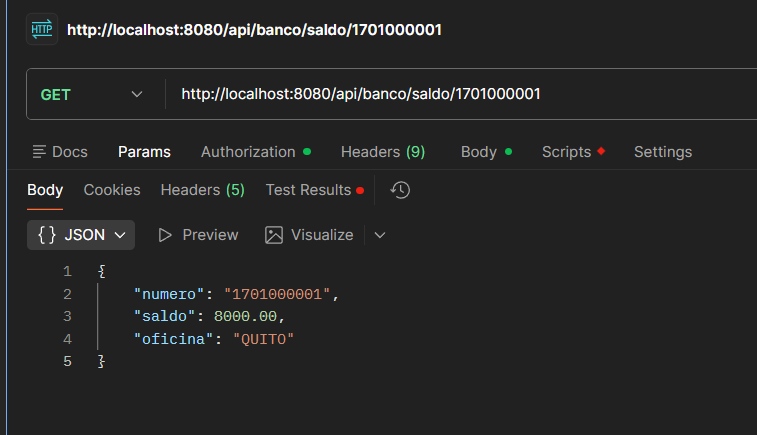
\includegraphics[width=0.7\textwidth]{images/image6.png}
    \caption{Respuesta JSON de Quito usando Postman.}
\end{figure}

\FloatBarrier
\subsection{Consulta distribuida de clientes}

Finalmente se ejecutó una consulta para obtener el listado completo de clientes registrados en ambas oficinas.

El servicio realizó dos consultas independientes, una hacia la base de datos de Cuenca y otra hacia la base de datos de Quito. Posteriormente, los resultados fueron combinados y enviados como una única respuesta al usuario.

Esta prueba demuestra el funcionamiento de una consulta distribuida, ya que la información proviene de diferentes nodos físicos, pero es presentada de forma transparente como un único conjunto de datos.

Endpoint utilizado: \texttt{GET /api/banco/clientes}

\begin{figure}[h!]
    \centering
    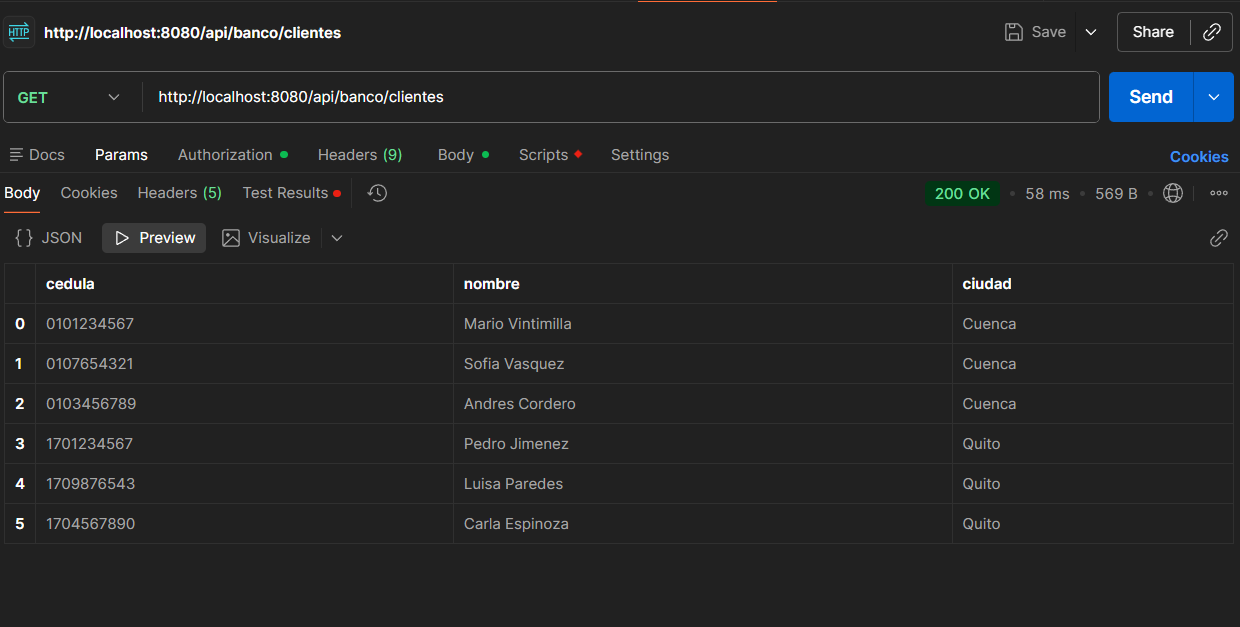
\includegraphics[width=0.85\textwidth]{images/image7.png}
    \caption{Respuesta JSON con los seis clientes con Postman.}
\end{figure}

% ===================== CONCLUSIONES =====================
\FloatBarrier
\section{Conclusiones}

\begin{enumerate}[leftmargin=*]
    \item La implementación permitió comprobar el funcionamiento de una base de datos distribuida mediante el uso de dos nodos PostgreSQL independientes administrados con Docker.
    \item El uso de múltiples DataSource en Spring Boot facilitó la conexión simultánea a diferentes bases de datos, permitiendo seleccionar automáticamente el nodo correspondiente según el prefijo del número de cuenta.
    \item Las pruebas realizadas demostraron que las consultas fueron ejecutadas correctamente tanto para el nodo de Cuenca como para el de Quito, además de validar la unión de información proveniente de ambos servidores.
    \item La práctica permitió comprender la importancia de las bases de datos distribuidas para mejorar la organización de la información y facilitar el acceso transparente a datos almacenados en diferentes ubicaciones.
\end{enumerate}

% ===================== BIBLIOGRAFÍA =====================
\FloatBarrier
\section{Bibliografía}

\begin{itemize}[leftmargin=*]
    \item Docker Inc. (2025). \textit{Docker Documentation}. \url{https://docs.docker.com/}
    \item PostgreSQL Global Development Group. (2025). \textit{PostgreSQL Documentation}. \url{https://www.postgresql.org/docs/}
    \item Spring. (2025). \textit{Spring Boot Reference Documentation}. \url{https://docs.spring.io/spring-boot/docs/current/reference/html/}
    \item Özsu, M. T., \& Valduriez, P. (2020). \textit{Principles of Distributed Database Systems} (4th ed.). Springer.
\end{itemize}

\end{document}
